\documentclass[12pt]{beamer}
\usepackage[utf8]{inputenc}
%\usepackage[latin1]{inputenc}
\usepackage[spanish]{babel}
%\usetheme{Warsaw}
%\usepackage{euler}
\usepackage{amsmath}
\usepackage{amsthm}
\usepackage{multicol}
\usepackage{graphicx}
\usepackage{tikz}
\usepackage{color}
\usepackage{hyperref}
\usepackage{listings}
\lstset{ %
language=Python,                % choose the language of the code
basicstyle=\small,       % the size of the fonts that are used for the code
numbers=left,                   % where to put the line-numbers
numberstyle=\footnotesize,      % the size of the fonts that are used for the line-numbers
stepnumber=1,                   % the step between two line-numbers. If it is 1 each line will be numbered
numbersep=5pt,                  % how far the line-numbers are from the code
backgroundcolor=\color{white},  % choose the background color. You must add \usepackage{color}
showspaces=false,               % show spaces adding particular underscores
showstringspaces=false,         % underline spaces within strings
showtabs=false,                 % show tabs within strings adding particular underscores
frame=single,   		% adds a frame around the code
tabsize=2,  		% sets default tabsize to 2 spaces
captionpos=b,   		% sets the caption-position to bottom
breaklines=true,    	% sets automatic line breaking
breakatwhitespace=false,    % sets if automatic breaks should only happen at whitespace
escapeinside={\#}{)}          % if you want to add a comment within your code
}
%\usepackage{epstopdf}
\DeclareGraphicsExtensions{.pdf,.png,.jpg}
\renewcommand {\arraystretch}{1.5}
\mode<presentation>
{
  \usetheme{Warsaw}
  \setbeamercovered{transparent}
  % or whatever (possibly just delete it)
}
\title{Ejercicio del m\'{e}todo de Horner}
\subtitle{Curso de F\'{i}sica Computacional}
\author{M. en C. Gustavo Contreras May\'{e}n}
\date{}
%\email{curso.fisica.comp@gmail.com}
%\ptsize{10}
\begin{document}
\maketitle
\fontsize{14}{14}\selectfont
\spanishdecimal{.}
\begin{frame}
\frametitle{Completa la siguiente tabla, usando el m\'{e}todo de Horner}
\[ P(x)=2 + 4 x - 5 x^{2} + 2 x^{3} - 6 x^{4} + 8 x^{5} + 10 x^{6}\]
Eval\'{u}a el polinomio $P(x)$ en:
\\
\medskip
\begin{center}
\begin{tabular}{l @{} | c}
x & P(x) \\
\hline -1.5 & \\
\hline -0.65 & \\
\hline 0.1 & \\
\hline 1.4 & \\
\hline 2.87 & 
\end{tabular}
\end{center}
\end{frame}
\begin{frame}
\frametitle{Estrategia}
\begin{enumerate}[<+->]
\item Una primera soluci\'{o}n es proporcionar al algoritmo el valor del punto a evaluar, esto funciona si son pocos puntos de la tabla.
\item La otra opci\'{o}n es manejar todos los datos que se van a evaluar dentro de una tabla, trabajemos de \'{e}sta manera.
\end{enumerate}
\end{frame}
\begin{frame}[fragile]
\frametitle{Primera estrategia}
\begin{lstlisting}
n=6
coeficiente = [2,4,-5,2,-6,8,10]

z = eval(raw_input('Escribe el valor de x a evaluar en el polinomio: '))

b = coeficiente[6]

while n >0 :
    n = n - 1    
    b = coeficiente[n] + z * b
  
print 'El valor del polinomio evaluado en ', z, ' es = ', b
\end{lstlisting}
\end{frame}
\begin{frame}[fragile]
\frametitle{Segunda estrategia}
\begin{lstlisting}
x0=[-1.5, -0.65, 0.1, 1.4, 2.87]

a=[2,4,-5,2,-6,8,10]   
\end{lstlisting}
Al manejar las listas, debemos de revisar con cuidado la manera en que se van a usar los elementos de ellas, ya que para el arreglo $x0$ que contiene los puntos a evaluar, \textcolor{blue}{debe de hacerse de izquierda a derecha}, mientras que en el m\'{e}todo de Horner, los \textcolor{red}{coeficientes se usan de derecha a izquierda}.
\end{frame}
\begin{frame}[fragile]
Tomamos entones primero un punto de $x0$ y se aplica el m\'{e}todo de Horner, por lo que se usar\'{a}n dos ciclos anidados.
\begin{lstlisting}
for i in range(len(x0)):
    Poli=0
    for n in range(len(a)-1,-1,-1):
        Poli=a[n] + Poli * x0[i]
    print "Poli(%.2f) = %f" %(x0[i],Poli)
\end{lstlisting}
\end{frame}
\begin{frame}[fragile]
\frametitle{Salida del c\'{o}digo}
\begin{tabular}{l c l}
P(-1.50) & = &  0.781250 \\
P(-0.65) & = & -4.506831 \\
P(0.10) & = &  2.351490 \\
P(1.40) & =  & 98.559680 \\
P(2.87) & = & 6758.702451
\end{tabular}
\end{frame}
\begin{frame}[fragile]
\frametitle{Mejoras adicionales al c\'{o}digo}
Como hemos resuelto el problema que se nos ped\'{i}a
\\
\medskip
\begin{center}
\begin{tabular}{l @{} | l}
x & P(x) \\
\hline -1.5 & 0.781250 \\
\hline -0.65 & -4.506831 \\
\hline 0.1 & 2.351490 \\
\hline 1.4 & 98.559680 \\
\hline 2.87 & 6758.702451
\end{tabular}
\end{center}
\end{frame}
\begin{frame}[fragile]
Podemos hacer unas mejoras aprovechando lo que ya vimos en el Tema 0, con funciones que nos agrupen el trabajo de las operaciones:
\begin{lstlisting}
def metodoHorner(x):
    metHorner = 0
    for n in range(len(a)-1,-1,-1):     
        metHorner = a[n] + metHorner * x
    return metHorner
\end{lstlisting}
\end{frame}
\begin{frame}[fragile]
Y como queremos comparar los valores obtenidos contra el polinomio, necesitamos otra funci\'{o}n que eval\'{u}e el mismo, en el intervalo de puntos, para ello usamos:
\begin{lstlisting}
def evaluaPoli(x):
    return 2 + x *(4 + x * (-5 + x * (2 + x *(-6 + x * (8 + x * 10)))))
\end{lstlisting}
\end{frame}
\begin{frame}[fragile]
Para graficar los puntos obtenidos por el m\'{e}todo de Horner y por la evaluaci\'{o}n directa del polinomio, vamos a ocupar el m\'{o}dulo de \texttt{numpy} y la librer\'{i}a de \texttt{mattplotlib}:
\\
\medskip
\verb|import matplotlib.pyplot as plt|
\verb|from numpy import *|
\end{frame}
\begin{frame}[fragile]
El c\'{o}digo completo queda:
\begin{lstlisting}
import matplotlib.pyplot as plt
from numpy import *

def metodoHorner(x):
...

def evaluaPoli(x):
...

x = linspace(-2.,3.)
plt.plot(x,metodoHorner(x),'ro')
plt.plot(x,evaluaPoli(x))
plt.grid(True)
plt.show()
\end{lstlisting}
\end{frame}
\begin{frame}[fragile]
\begin{figure}
	\centering
	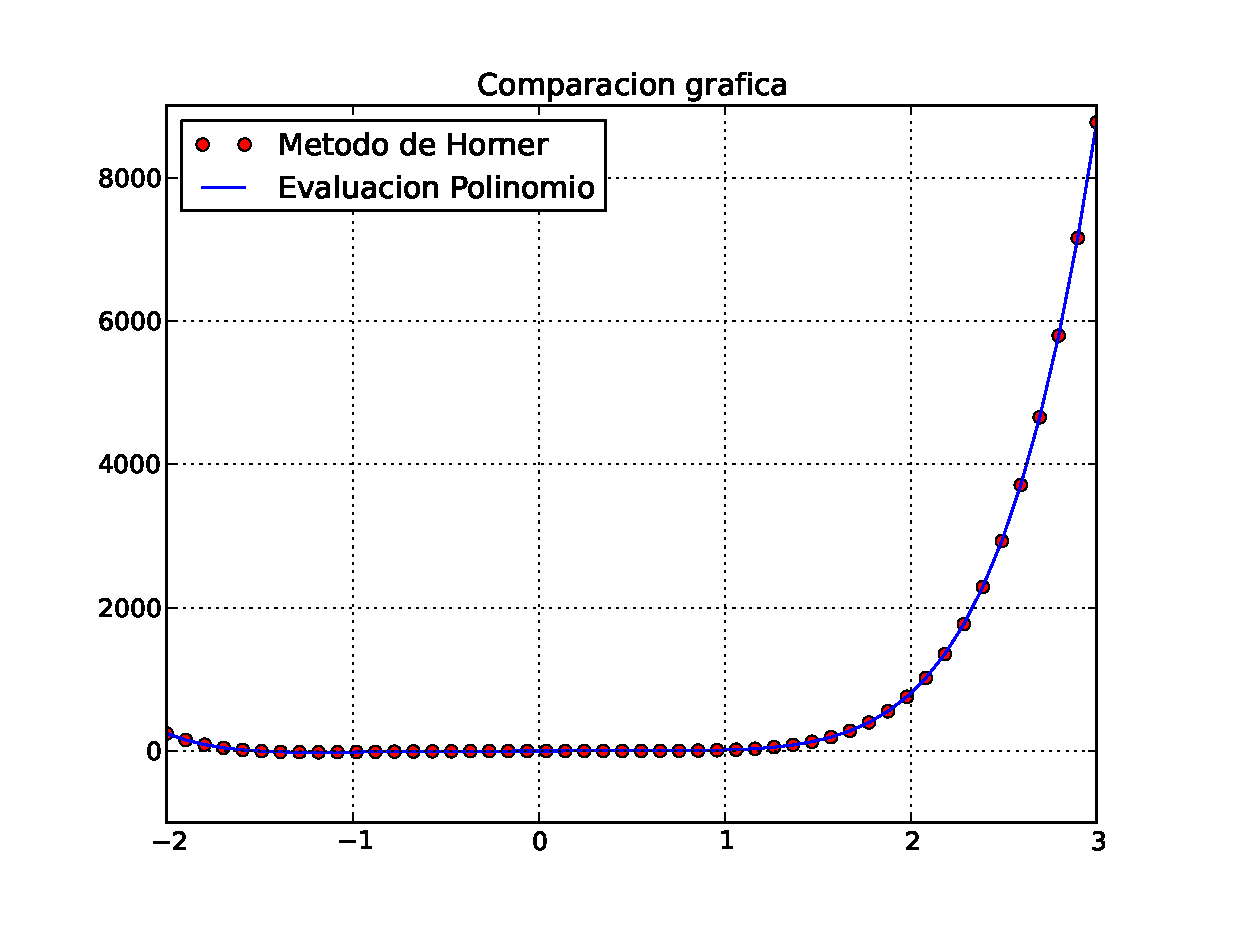
\includegraphics[scale=0.5]{MetodoHorner.eps} 
\end{figure}
\end{frame}
\end{document}